\chapter{Vision and Technical Strategy}

The development of a large software system is a very critical process and there are a lot of parts that are involved in a project that needs to follow key software development paradigms so that it is easy to maintain. Its not just about writing code, its about creating a system that is bug free, easy to maintain, scalable and efficient.

Since an already built large software system is quite complex, so understanding this system requires certain strategies and tools.~\citep{Folmer2005} discusses about the useability issues in the software systems post-development and they require significant architectural changes. In order to deal with such architectural changes, understanding of the whole system is required and if the system is large enough, major resources are spent to fix even minor issues. 

~\citep{SeMaintainance2001} states that several surveys indicate that software maintenance consumes 60\% to 80\% of the total life cycle costs. Also the maintenance costs are largely due to enhancement (often 75{-}80\%), rather than corrections. So a framework should be developed that could solve these issues by doing reverse engineering on the software systems and showing the importants aspects of the software architecture in order to make it easy to understand and perform the required tasks.

\begin{figure}[ht]
    \centering
    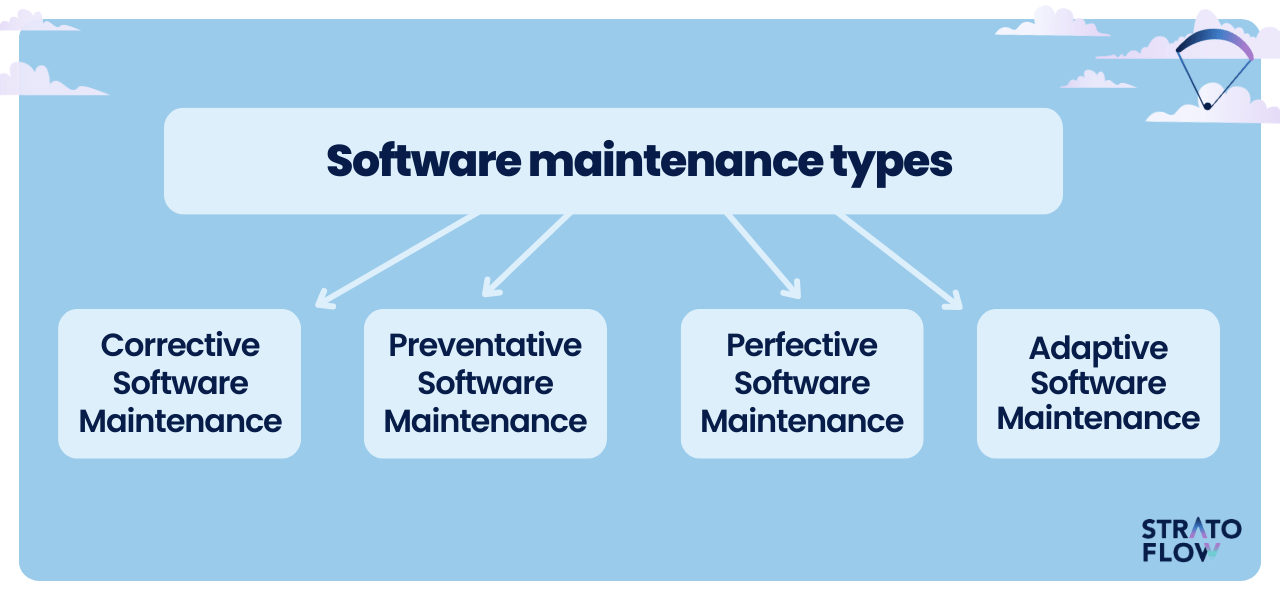
\includegraphics[width=0.8\textwidth]{figures/se_maintenance.png}
    \caption[Software Maintenance Types]{Software Maintenance Types (adapted from~\cite{stratoflow2025})}
	\label{fig_se_maintenance}
\end{figure}

\section{Vision}

Keeping in mind the above discussed issues, there is a need for an approach in which the software system could be analyzed, undergo processing and produce useful informations that can be used to provide enhanced insights about the project. The vision is to use a framework consisting of 3 components: 
\nameref{subsec:component-probes}, \nameref{subsec:component-sst} and \nameref{subsec:component-visualizer}. All three components will be discussed in detail in section{ }\ref{sec:tech-strategy}.

In this report, we will discuss,implement and validate this framework by extrac
ting static information from a project. In the future, this can be implemented/integrated with the CI/CD pipeline and provide dynamic information from the projects. The test project used in this report is Java spring framework based project called petclinic. Read more about this project from \href{https://github.com/spring-petclinic/spring-petclinic-microservices}
{spring petclinic microservices github repository}~\citep{spring-petclinic}.

Moreover, our approach will be mainly focused on the unified data source (UDS) approach.~\citep{unifiedData2025} states that Unified Data refers to the integration and consolidation of data from various sources into a single, cohesive framework. This approach allows organizations to streamline their data management processes, ensuring that all data is accessible and usable across different departments and applications. By unifying data, businesses can eliminate silos, reduce redundancy, and enhance the overall quality of their data analytics efforts. It means that consistent, up-to-date and valid data will be available using the UDS technique.


\section{Technical Strategy}\label{sec:tech-strategy}

\subsection{Framework Components}\label{subsec:framework-components}

The framework contains three main components.
\begin{itemize}
    \item \nameref{subsec:component-probes}
    \item \nameref{subsec:component-sst}
    \item \nameref{subsec:component-visualizer}
\end{itemize}


\subsection{Probes}\label{subsec:component-probes}

The first component of the framework consists of \textbf{probes}. Probes represent distinct informational artifacts that are systematically extracted from software systems to provide insights and actionable data. In the context of this report, we have identified and extracted specific pieces of information that are detailed in the below subsections. These probes serve as the foundational elements for gathering critical data points that enable analysis and decision-making. 

Looking forward, this concept can be expanded to more complex and targeted informational needs. By refining the scope and nature of the probes, we can tailor the probes according to our needs and to capture more refined data, addressing evolving requirements and insights that drive meaningful outcomes. This flexibility ensures that as the systems grow or change, the framework remains relevant and capable of producing deeper, more impactful information.

\begin{itemize}[leftmargin=*, label=$\bullet$]

    \item \subsubsection*{Authors Contributions}
    What it is?, why we need it, what it solved? type of data extracted... 
    \item \subsubsection*{File Authors}
    What it is?, why we need it, what it solved? type of data extracted... 
    \item \subsubsection*{Microservices Endpoints}
    What it is?, why we need it, what it solved? type of data extracted... 

\end{itemize}

\subsection{Single Source of Truth (SST)}\label{subsec:component-sst}
\subsection{Visualizer}\label{subsec:component-visualizer}

If you need to use quotes, type it ``like this''.

\section{Referencing}
These are some sample references to GAMYGDALA~\citep{popescu2014gamygdala} from 
the \texttt{references.bib} file and state effects of 
cognition~\citep{hudlicka2002time} from the \texttt{references\_another.bib} 
file. These references are not in the same .bib file.

\section{Figures}
This is a single image figure (Figure~\ref{fig_singleenv}):

\begin{figure}[ht]
    \centering
    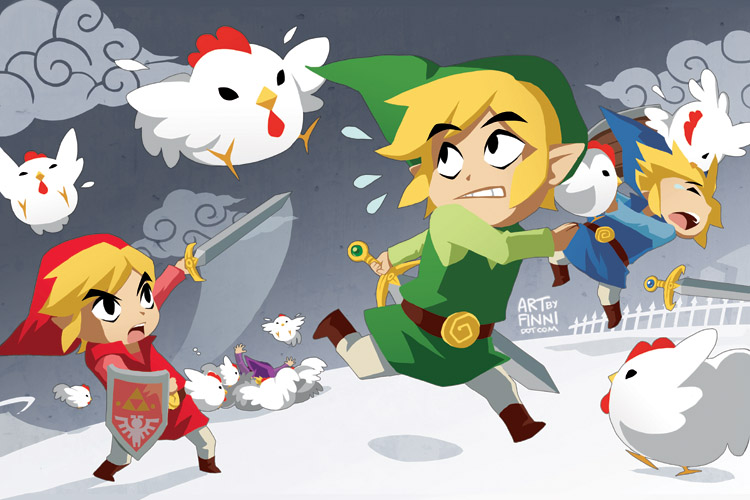
\includegraphics[width=0.6\textwidth]{figures/Sample/tumblr_static_eaceks0rfxsss8o4swscw40wo.jpg}
    \caption[Single Figure Environment Listed Title]{This is a single figure 
    environment}
    \label{fig_singleenv}
\end{figure}

This is a multi-image figure with a top (Figure~\ref{fig_multienv_1}) and bottom (Figure~\ref{fig_multienv_2}) aligned subfigures:

\begin{figure}[ht]
	\centering
	\begin{subfigure}[t]{\textwidth}
		\centering
		
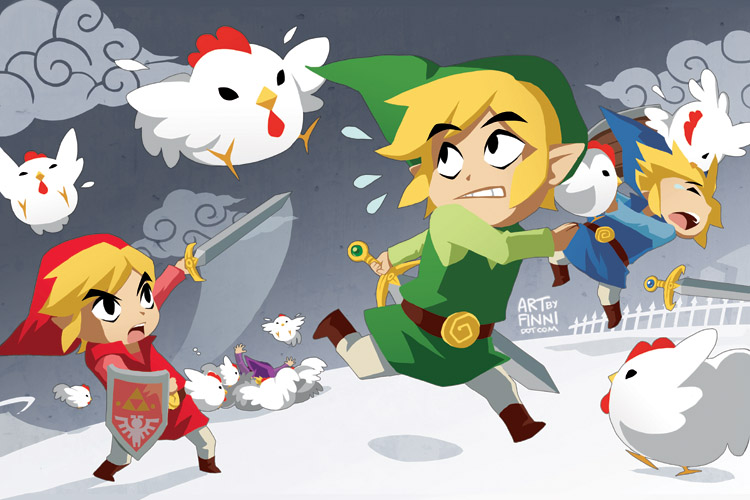
\includegraphics[width=0.7\textwidth]{figures/Sample/tumblr_static_eaceks0rfxsss8o4swscw40wo.jpg}
		\caption{Figure 1}
		\label{fig_multienv_1}
	\end{subfigure}
	~
	\begin{subfigure}[t]{\textwidth}
		\centering
		
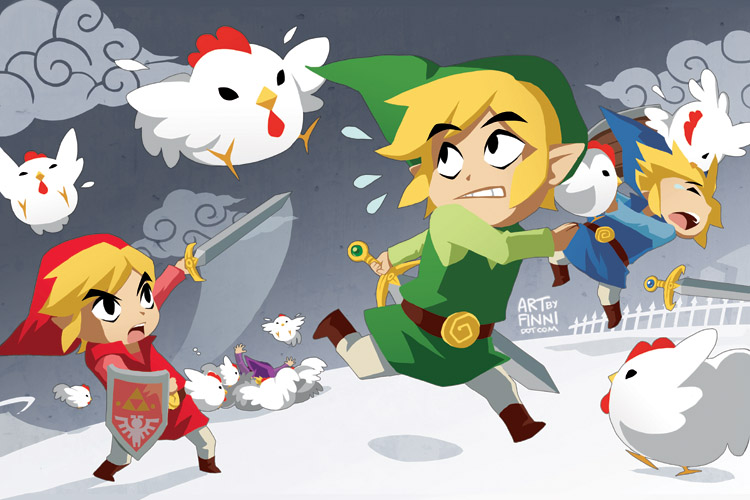
\includegraphics[width=0.7\textwidth]{figures/Sample/tumblr_static_eaceks0rfxsss8o4swscw40wo.jpg}
		\caption{Figure 2}
		\label{fig_multienv_2}
	\end{subfigure}
	
	\caption{A Multi-Figure Environment}
	\label{fig_multienv}
\end{figure}

\section{Tables}

Here is a sample table (Table~\ref{tab_sample}):

	\begin{table}[ht]
	\centering
	\begin{tabular}{ m{0.2\textwidth} m {0.1\textwidth} m{0.15\textwidth} }
		\toprule
		A & $\longleftrightarrow$ & B \\
		C & $\longleftrightarrow$ & D \\
		\bottomrule	
	\end{tabular}	
	\caption{A sample table}	
	\label{tab_sample}
\end{table}

\subsection{Long Tables}
A sample long table is shown in Appendix~\ref{appendix_b}.

\section{Equations}

Here is a sample equation (Equation~\ref{eq_lineslope}):

\begin{equation} \label{eq_lineslope}
	y = mx + b
\end{equation}